% *********************************************************************
% © 2016–2026 Jeremy Sylvestre
%
% Permission is granted to copy, distribute and/or modify this document
% under the terms of the GNU Free Documentation License, Version 1.3 or
% any later version published by the Free Software Foundation; with no
% Invariant Sections, no Front-Cover Texts, and no Back-Cover Texts. A
% copy of the license is included in the appendix entitled “GNU Free
% Documentation License” that appears in the output document of this
% PreTeXt source code. All trademarks™ are the registered® marks of
% their respective owners.
%
% *********************************************************************
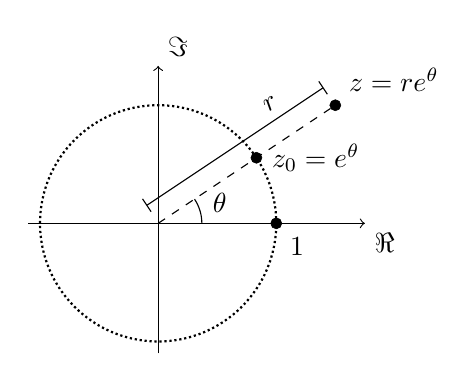
\begin{tikzpicture}[
	scale=1.5,
	point/.style={circle,draw,very thin,fill,inner sep=0pt,minimum size=4pt},
]
	\draw[->] (-1.1,0) to (1.75,0) node[below right] {$\Re$};
	\draw[->] (0,-1.1) to (0,1.333) node[above right] {$\Im$};

	\node[point] at (1,0) [label=below right:{$1$}] {};

	\node[point] at (1.5,1) (z) [label=above right:{$z = re^{\ci\theta}$}] {};
	\node[point] at (0.832,0.555) [label=right:{$z_0 = e^{\ci\theta}$}] {};

	\draw[dashed] (0,0) to (z);

	\draw (0,0) ++(0:0.37cm) arc (0:33.69:0.37cm) node[midway,xshift=0.25cm,yshift=0.1cm] {$\theta$};

	\draw[densely dotted, thick] (0,0) circle (1cm);

	\draw[|-|,thin,xshift=-0.1cm,yshift=0.15cm]
		(0,0) to node[above,sloped,near end] {$r$} (1.5,1);

\end{tikzpicture}
